% Fig. 1 -- how an inference Job gets the n150 (report Sec. 3.4). Precedent: G09 (system boundary, numbered steps).
% Structure spec (every part traced to ~/Desktop/n150 @ 8387795 or k8s-llm-example @ 0bb1d0f):
%   outside: User (kubectl, chat.py)                                 README.md, k8s-llm-example/README.md
%   Node tenstorrent (KVM VM, kubeadm) (boundary)                    config/kubeadm.yaml, single node
%     kube-apiserver + MAP (n150-job-defaults, n150-board)          config/job-defaults.yaml
%     kube-scheduler (allocates DRA claims)                          resource.k8s.io/v1
%     Kueue (ClusterQueue default, deviceClassMappings)              config/kueue.yaml, config/kueue-values.yaml
%     kubelet + containerd (CDI)                                     scripts/node.sh, config/containerd.toml
%     tt-operator (group, Helm chart 0.3.0)                          scripts/cluster.sh, config/tt-operator-values.yaml
%       tt-dra-driver kubelet plugin, tt-telemetry
%     Inference Pod (namespace u-<user>)                             n150/llm.yaml
%       server container > vLLM, TT-NN / tt-metal
%       init container cleanup-hugepages                             config/job-defaults.yaml (n150-board)
%     Prometheus                                                     config/monitoring-values.yaml
%     n150 (Wormhole, PCIe)                                          lspci 1e52:401e
%   omitted (stated in the caption): tt-fabric-manager, node-feature-discovery (both deployed by tt-operator)
%   edges: dashed = Kubernetes control (API objects, kubelet gRPC); solid = HTTP (inference API, metrics scrape);
%          heavy = device access (/dev/tenstorrent/0, tt-kmd); tt-telemetry -> n150 from its device metrics
%          (raw/env/tt-telemetry-metric-names.txt: tt_asic_temperature_celsius, tt_device_accessible, ...)
%          ResourceSlice: written by the driver to the API server, read by the scheduler (label says so)
%   steps: 1 submit Job; 2 Kueue admits (charges tenstorrent.com/chip 1); 3 scheduler allocates tt-0 to the ResourceClaim;
%          4 NodePrepareResources writes the CDI spec; 5 containerd starts the Pod with the device; 6 inference requests
\documentclass[tikz,border=2pt]{standalone}
\usepackage[T1]{fontenc}
\usepackage{helvet}
\renewcommand{\familydefault}{\sfdefault}
\usetikzlibrary{positioning,arrows.meta,fit,backgrounds,calc,matrix}

\definecolor{accent}{HTML}{1F3A5F}
\definecolor{unitfill}{HTML}{DAE3F3}
\definecolor{poolfill}{HTML}{F2F2F2}
\definecolor{hwfill}{HTML}{FFF2CC}
\definecolor{muted}{HTML}{6B7280}

\tikzset{
  every picture/.style={line width=0.5pt},
  lab/.style={font=\fontsize{7}{8.4}\selectfont},
  title/.style={font=\fontsize{7.5}{9}\selectfont\bfseries},
  comp/.style={draw, fill=white, rounded corners=1.5pt, align=center, minimum height=22pt, minimum width=84pt, inner sep=2pt, lab},
  inner/.style={comp, minimum width=70pt, minimum height=13pt},
  hw/.style={comp, fill=hwfill, line width=1pt},
  unit/.style={draw, fill=unitfill, rounded corners=2pt},
  pool/.style={draw, fill=poolfill},
  group/.style={draw=accent, dash pattern=on 2pt off 1.5pt, rounded corners=2pt},
  boundary/.style={draw=muted, inner sep=7pt},
  ext/.style={comp, fill=muted!12, minimum width=44pt},
  ctrl/.style={dash pattern=on 2pt off 1.5pt, -{Stealth[length=3pt, width=2.4pt]}},
  req/.style={-{Stealth[length=3pt, width=2.4pt]}},
  data/.style={line width=1.1pt, {Stealth[length=3.6pt, width=3.6pt]}-{Stealth[length=3.6pt, width=3.6pt]}},
  stepnum/.style={circle, fill=accent, text=white, inner sep=0pt, minimum size=8pt, font=\fontsize{6}{6}\selectfont\bfseries},
  node distance=34pt and 36pt,
}

\begin{document}
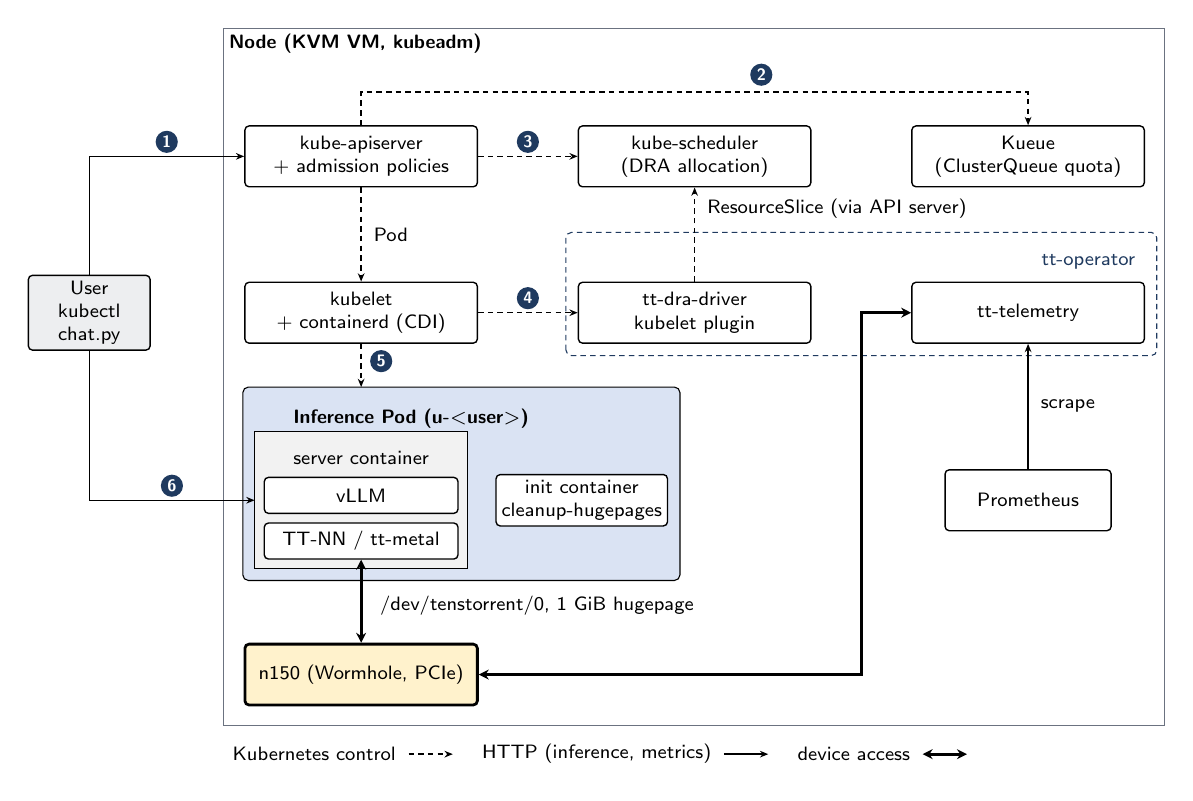
\begin{tikzpicture}
  % control plane (top row) and node agents (second row): placed relative to kube-apiserver
  \node[comp] (api) {kube-apiserver\\+ admission policies};
  \node[comp, right=of api] (sched) {kube-scheduler\\(DRA allocation)};
  \node[comp, right=of sched] (kueue) {Kueue\\(ClusterQueue quota)};
  \node[comp, below=of api] (kubelet) {kubelet\\+ containerd (CDI)};
  \node[comp, right=of kubelet] (drv) {tt-dra-driver\\kubelet plugin};
  \node[comp, right=of drv] (tel) {tt-telemetry};
  % inference Pod: server container (framework over TT-NN) and the injected init container
  \node[inner, below=48pt of kubelet] (fw) {vLLM};
  \node[inner, below=3pt of fw] (ttnn) {TT-NN / tt-metal};
  \node[lab, above=1pt of fw] (srvlabel) {server container};
  \node[fit=(srvlabel)(fw)(ttnn), inner sep=3pt] (srv) {};
  \node[inner, minimum width=58pt, right=10pt of srv.east] (init) {init container\\cleanup-hugepages};
  \node[title, above=1pt of srvlabel.north west, anchor=south west] (podtitle) {Inference Pod (u-\textless user\textgreater)};
  \node[fit=(podtitle)(srv)(init), inner sep=4pt] (pod) {};
  \node[comp, minimum width=60pt] (prom) at (tel |- srv) {Prometheus};
  \node[hw, below=30pt of ttnn] (n150) {n150 (Wormhole, PCIe)};
  % tt-operator: the parts it deploys, one group
  \node[lab, text=accent, above=1pt of tel.north east, anchor=south east] (optitle) {tt-operator};
  \node[fit=(drv)(tel)(optitle), inner sep=4pt] (op) {};
  \coordinate (top) at ($(api.north)+(0,12pt)$);
  \coordinate (headroom) at ($(top)+(0,16pt)$);   % title row above the step-2 route
  \node[boundary, fit=(api)(kueue)(tel)(pod)(prom)(n150)(headroom)] (node) {};
  \node[title, anchor=north west, inner sep=2pt] at (node.north west) {Node (KVM VM, kubeadm)};
  \begin{scope}[on background layer]
    \draw[unit] (pod.south west) rectangle (pod.north east);
    \draw[pool] (srv.south west) rectangle (srv.north east);
    \draw[group] (op.south west) rectangle (op.north east);
  \end{scope}
  \node[ext, left=26pt of node.west |- kubelet] (user) {User\\kubectl\\chat.py};

  % 1 submit, 6 inference: from the user, across the boundary
  \draw[req] (user.north) |- node[stepnum, pos=.75, above=1pt] {1} (api.west);
  \draw[req] (user.south) |- node[stepnum, pos=.75, above=1pt] {6} (srv.west);
  % control path
  \draw[ctrl] (api.north) -- (api.north |- top) -| node[stepnum, pos=.3, above=2pt] {2} (kueue.north);
  \draw[ctrl] (api.east) -- node[stepnum, above=1pt] {3} (sched.west);
  \draw[ctrl] (drv.north) -- node[lab, right=1pt, pos=.78] {ResourceSlice (via API server)} (sched.south);
  \draw[ctrl] (api.south) -- node[lab, right=1pt] {Pod} (kubelet.north);
  \draw[ctrl] (kubelet.east) -- node[stepnum, above=1pt] {4} (drv.west);
  \draw[ctrl] (kubelet.south) -- node[stepnum, right=3pt, pos=.4] {5} (kubelet.south |- pod.north);
  % device access
  \draw[data] (ttnn.south) -- node[lab, right=3pt, pos=.55] {/dev/tenstorrent/0, 1 GiB hugepage} (n150.north);
  \coordinate (lane) at ($(drv.east)!0.5!(tel.west)$);
  \draw[data] (n150.east) -| (lane |- tel) -- (tel.west);
  % metrics
  \draw[req] (prom.north) -- node[lab, right=1pt] {scrape} (tel.south);

  % legend row
  \node[lab, anchor=north west] (l1) at ($(node.south west)+(0,-4pt)$) {Kubernetes control};
  \draw[ctrl] ($(l1.east)+(1pt,0)$) -- ++(16pt,0);
  \node[lab, anchor=west] (l2) at ($(l1.east)+(24pt,0)$) {HTTP (inference, metrics)};
  \draw[req] ($(l2.east)+(1pt,0)$) -- ++(16pt,0);
  \node[lab, anchor=west] (l3) at ($(l2.east)+(24pt,0)$) {device access};
  \draw[data] ($(l3.east)+(1pt,0)$) -- ++(16pt,0);
\end{tikzpicture}
\end{document}
